%!xelatex = 'xelatex --halt-on-error %O %S'

\documentclass{seuer}
\usepackage{listings}
\begin{document}

% 标题,作者
\emptitle{数字信号处理大作业}
\empauthor{自动化学院}{220221878 邱洪彬}{}
% 奇数页页眉 % 请在这里写出第一作者以及论文题目
\fancyhead[CO]{{\footnotesize 邱洪彬: 数字信号处理大作业}}
%\Keyword{关键词, 很关键的词, 十分关键的词, 有一些关键的词, 大关键词}

\maketitle

%%%%%%%%摘要
%\begin{empAbstract}
%这是摘要
%\end{empAbstract}

%%%%%%%%首页角注,依次为实验时间、报告时间、学号、email
\empfirstfoot{2022.12至2023.2}{}{220221878}{}


% 如果首页脚注有重复就调整下一行的数值直到正常
\enlargethispage{-1.3cm} 
\wuhao 
%  分栏开始

\section{综述题}
\subsection{第一题}
设计一个声音信号采集、滤波和频谱分析的技术方案,尽量考虑各种因
素的影响,例如采样率、截止频率等,并尽量考虑减少频谱泄漏、提高频谱
分辨率等的措施。
\\解答:人能够听到的的声音频率范围为20-20kHz,超过这全范围的声音就听不到了,因此采集的声音信号可以假定都位于这个频率范围内。根据采样定理,采样频率应该为信号最高频率的两倍,这样才不会在频域产生频率混叠,同时考虑实际情况留出余量,采样频率设为48kHz。
\\假定环境中的噪声主要由高频成分构成,设计低通滤波器,并采用合适的截止频率可以完成对采集信号的降噪处理。在采集信号时,不可能持续不断的处理无限长的序列,因此需要对信号进行截断,但是当采集的信号不是周期信号或者截断的长度不是完整周期的整数倍时,将会造成频谱泄露,为了减轻这种影响,采用汉宁窗等主瓣宽度大,旁瓣宽度小的窗进行截断,起到一定的过渡效果。
\\为了提高频谱分辨率,则需要增加采样时间,但这样一来又会增加采样点数,带来运算复杂度的增加,因此要结合实际情况选择合适的采样点数与采样频率,满足所需分辨率的要求。
\\经过Matlab仿真,本题从一首网络歌曲中截取一断信号进行处理。信号采样频率为44100Hz,时间长度为3秒。为了研究噪声的影响,考虑到人声范围为300-3400Hz,在信号中加入一段4500Hz的正弦噪声,滤波器采用切比雪夫滤波器,设计通带频率为4000Hz,阻带频率为4200Hz。将滤波器用于加入噪声后信号,观察滤波效果,如\ref{Fig1}所示。从频谱中可见,经过低通滤波器后,噪声被有效地滤除了,时域波形的信号也得到了较好的还原。
\begin{figure}[H] %H为当前位置,!htb为忽略美学标准,htbp为浮动图形
	\centering %图片居中
	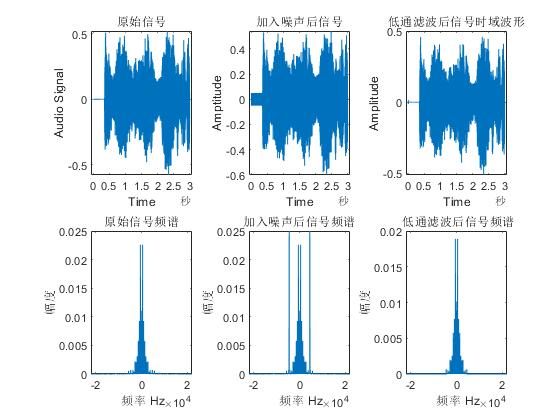
\includegraphics[width=1\textwidth]{"../DSPAssignment/Assignment1.jpg"} %插入图片,[]中设置图片大小,{}中是图片文件名
	\caption{Assignment1} %最终文档中希望显示的图片标题
	\label{Fig1} %用于文内引用的标签
\end{figure}
\subsection{第二题}
完成一个离散时间线性时不变系统的输入输出分析,并用 FFT 设计一个
算法流程完成一段时间的仿真验证(利用分段线性卷积完成)。
\\解答:假设所分析的离散时间线性时不变系统为:$y(n)-1.25 y(n-1)+0.375 y(n-2)=2 x(n)-3 x(n-1)+2 x(n-2)$,则其系统函数为:$H(z)=\frac{2-3z^{-1}+2z^{-2}}{1-1.25z^{-1}+0.375z^{-2}},ROC:|z|>0.75$。由于该系统是以差分方程形式给出的,因此其暗含线性和时不变特性。由其系统函数可知,其两个极点:$z_1=0.5,z_2=0.75$,均位于单位圆内部,因此该离散LTI系统是稳定的,同时由于因收敛域包含无穷远处,所以该系统也是因果性的 。
\\使用FFT实现该系统的卷积,由于该系统冲激响应是无限长序列,因此只用有限点长部分来近似代替,采用重叠相加法,将输入序列分段后用FFT转化到频域,将系统冲激响应也转化到频域,应用卷积定理,在时域卷积相当于在频域相乘,然后用IFFT转化到时域得到输出信号。重叠相加法主要过程如\ref{overlap}所示。
\begin{equation}\label{overlap}
	\begin{aligned}	
	h(n)&= \begin{cases}h(n), & 0 \leqslant n \leqslant M-1 \\ 0, & M \leqslant n \leqslant N-1\end{cases}
	\\x_i(n)&=\left\{\begin{array}{ll}x(n+i L), & 0 \leqslant n \leqslant L-1 \\ 0, & L \leqslant n \leqslant N-1\end{array}, \quad i=0,1, \cdots\right.
	\\H(k)&=\operatorname{DFT}[h(n)], \quad N 点
	\\X_i(k)&=\operatorname{DFT}\left[x_i(n)\right], \quad N 点 , i=0,1, \cdots
	\\Y_i(k)&=X_i(k) H(k), \quad i=0,1, \cdots
	\\y_i(n)&=\operatorname{IDFT}\left[Y_i(k)\right], \quad N 点, i=0,1, \cdots
	\\y(n)&=\sum_{i=0}^{\infty} y_i(n-i L), \quad \text{重叠部分相加}
    \end{aligned}
\end{equation}
经过Matlab仿真验证(代码如下),结果如图\ref{Fig2}所示,从中可以看出用重叠相加法并用FFT实现的变换过程的方法所得到的输出与直接卷积计算得到到结果一致,所以对该系统完成了验证。
\lstset{language=Matlab}
\begin{lstlisting}
	m=5;
	x=[1 zeros(1,m-1)];
	b=[2 -3 2];
	a=[1 -1.25 0.375];
	K=0:1:m-1;
	y=filter(b,a,x);%由系统函数得到冲激响应
	subplot(221)
	stem(K,y);
	title( '冲激响应' );
	xlabel( 'n' );
	ylabel( 'h(n)' );
	h_n = y;
	x_k = [1, 2, 3, 4, 5, 6, 7];
	M = 5;
	L = 7;
	for k = 1:4
	x_n((k-1)*L+1:L*k) = x_k;%构造输入序列
	end
	subplot(223)
	stem(0:length(x_n)-1,x_n)
	title( '输入序列' );
	xlabel( 'n' );
	ylabel( 'x(n)' );
	H_k = fft(h_n, M+L-1);
	y_n = zeros(1, M+L*4-1);
	y_n(1: L+M-1) = ifft(fft(x_n(1:L), M+L-1).*H_k);%重叠相加法+FFT计算输出序列
	for k = 2:4
	y_k = ifft(fft(x_n((k-1)*L+1:k*L),M+L-1).*H_k);
	y_n((k-1)*L+1:(k-1)*L+M-1) = y_k(1:M-1)+y_n((k-1)*L+1:(k-1)*L+M-1);
	y_n((k-1)*L+M:k*L+M-1) = y_k(M:L+M-1);
	end
	subplot(222)
	stem(0:length(y_n)-1,y_n)
	title( '重叠相加法输出序列' );
	xlabel( 'n' );
	ylabel( 'y(n)' );
	y_i = conv(x_n,h_n);%直接计算卷积与结果相比较
	subplot(224)
	stem(0:length(y_i)-1,y_i)
	title( '直接卷积计算输出序列' );
	xlabel( 'n' );
	ylabel( 'y(n)' );
\end{lstlisting}
\begin{figure}[H] %H为当前位置,!htb为忽略美学标准,htbp为浮动图形
	\centering %图片居中
	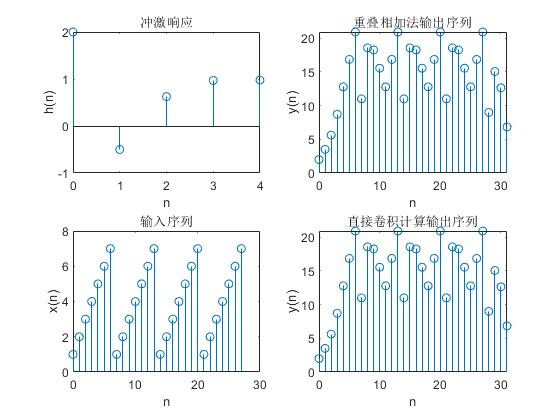
\includegraphics[width=0.8\textwidth]{"../DSPAssignment/Assignment2.jpg"} %插入图片,[]中设置图片大小,{}中是图片文件名
	\caption{Assignment2} %最终文档中希望显示的图片标题
	\label{Fig2} %用于文内引用的标签
\end{figure}
\subsection{第三题}
设计一个正弦波或方波的离散时间信号发生器,分析其系统函数 H(z),
利用其实现结构给出仿真结果。
\\解答:使用符号函数来实现信号发生器,$y(n)=Asign(x(n))$,当$x(n)=sin(2\pi fnT)$时,可以实现方波信号的产生,当$x(n)=sin(2\pi fnT)\ge0, y(n)=A,x(n)=sin(2\pi fnT)<0, y(n)=-A$,同时由于输入信号$x(n)=sin(2\pi fnT)$在一个周期内正负信号持续时间相等,即可实现方波信号发生器。
\\该信号发生器的系统函数为$H(z)=\frac{A}{1-z^{-1}}$,由于该系统比较简单,使用直接型结构就可实现,如图\ref{Fig3}所示,用Simulink实现其结构如图\ref{simulink}所示,经过Matlab仿真验证,发现该信号发生器系统的确能够产生方波信号,结果如图\ref{Fig4}所示。
\begin{figure}[H] %H为当前位置,!htb为忽略美学标准,htbp为浮动图形
	\centering %图片居中
	\includegraphics[width=1\textwidth]{"符号函数.pdf"} %插入图片,[]中设置图片大小,{}中是图片文件名
	\caption{方波发生器直接型结构} %最终文档中希望显示的图片标题
	\label{Fig3} %用于文内引用的标签
\end{figure}
\begin{figure}[H] %H为当前位置,!htb为忽略美学标准,htbp为浮动图形
	\centering %图片居中
	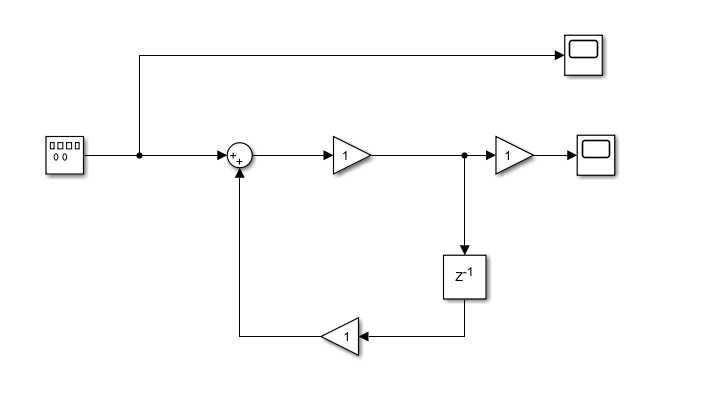
\includegraphics[width=1\textwidth]{"../DSPAssignment/方法发生器simulink.png"} %插入图片,[]中设置图片大小,{}中是图片文件名
	\caption{方波发生器直接型结构Simulink仿真} %最终文档中希望显示的图片标题
	\label{simulink} %用于文内引用的标签
\end{figure}
\begin{figure}[H] %H为当前位置,!htb为忽略美学标准,htbp为浮动图形
	\centering %图片居中
	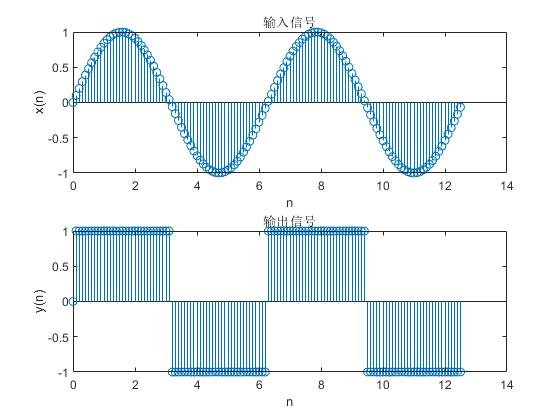
\includegraphics[width=1\textwidth]{"../DSPAssignment/Assignment3.jpg"} %插入图片,[]中设置图片大小,{}中是图片文件名
	\caption{Assignment3} %最终文档中希望显示的图片标题
	\label{Fig4} %用于文内引用的标签
\end{figure}
\section{实验大作业}
利用所学知识,采用两种滤波器设计方法(不变法和双线性法)设计一个低
通 IIR 滤波器,参数自定。要求:
\begin{enumerate}
	\item 能够给出设计过程的理论分析详实过程;
	\item 能够在 Matlab 里完成仿真验证;
	\item 针对仿真结果进行深入分析两种方法的优缺点;
	\item *各自找出一种方法对两种滤波器性能进行改善,并对比(可选)
\end{enumerate}
解答:IIR 滤波器差分方程的一般表达式为
$$
y(n)=\sum_{i=0}^N b_i x(n-i)-\sum_{i=1}^M a_i y(n-i)
$$
式中, $\mathrm{x}(\mathrm{n})$ 为输入序列; $\mathrm{y}(\mathrm{n})$ 为输出序列; $a_i$ 和 $b_i$ 为滤波器系数。
\subsection{理论计算}
\begin{enumerate}
	\item 脉冲响应不变法:\\$\omega=\Omega T$, 令 $T=1$,采用巴特沃斯滤波器设计法,$H^2|\Omega|=|H(j \Omega)|^2=\frac{1}{1+\left(\frac{j \Omega}{j \Omega c}\right)^{2 N}}$,取$\Omega_1=\frac{\omega}{T}=\frac{0.2613 \pi}{T}, \quad \Omega_2=\frac{\omega}{T}=\frac{0.4018 \pi}{T}$,根据巴特沃斯滤波器的表达式列出所需满足的条件,\\$\left\{\begin{array}{l}-10 \lg \left[1+\left(\frac{j \frac{0.2613 \pi}{T}}{j \Omega_c}\right)^{2 N}\right]=-0.75 \\ -10 \lg \left[1+\left(\frac{j \frac{0.4018 \pi}{T}}{j \Omega_c}\right)^{2 N}\right]=-20\end{array}\right.$,解得$\left\{\begin{array}{l}\Omega^{\prime}_c=\frac{0.2913 \pi}{T} \\ N^{\prime}=7.28\end{array}\right.$,\\取 $\mathrm{N}=8$, 则 $\Omega_\mathrm{c}=0.9472$
	\\由 $1+\left(\frac{S}{j \Omega_c}\right)^{2 N}=0$
	$\therefore$ 极点为 $\mathrm{S}_{\mathrm{k}}^{\prime}=\Omega_{\mathrm{c}} \mathrm{e}^{\mathrm{j}\left[\frac{2 \mathrm{k}-1}{16}+\frac{1}{2}\right] \pi}, \mathrm{k}=1,2, \ldots,16$
	\\最低阶巴特沃斯模拟滤波器系统函数的极点为左半平面的极点:
	$$
	\begin{gathered}
		\mathrm{S}_{\mathrm{k}}=\Omega_{\mathrm{c}} \mathrm{e}^{\mathrm{j}\left[\frac{2 \mathrm{k}-1}{16}+\frac{1}{2}\right] \pi}, \mathrm{k}=1,2, \ldots, 8 \\
		H(s)=\frac{\prod_{k=1}^8(-S_k)}{\prod_{k=1}^8(s-S_k)}=\frac{\Omega _c^8}{\prod_{k=1}^8(s-S_k)}=\sum_{k=1}^8 \frac{A_k}{s-S_k}
	\end{gathered}
	$$
	\\数字滤波器的系数函数为将 $\mathrm{S_k} \rightarrow \mathrm{e}^{\mathrm{S_kT}}$
	$$
	H(z)=\sum_{k=1}^8 \frac{A_k}{1-e^{S_k T} z^{-1}}
	$$
	\item 双线性变换法
	\\$\Omega=\frac{2}{T} \operatorname{tg} \frac{\omega}{2},
	取T=1$,滤波器采用巴特沃斯滤波器,取$\Omega_1=\frac{2}{T} \operatorname{tg} \frac{0.2613 \pi}{2}, \quad \Omega_2=\frac{2}{T} \operatorname{tg} \frac{0.4018 \pi}{2}$,则应满足条件为:$\left\{\begin{array}{l}-10 \lg \left[1+\left(\frac{j \frac{2}{T} \operatorname{tg} \frac{0.2613 \pi}{2}}{j \Omega_c}\right)^{2 N}\right]=-0.75 \\ -10 \lg \left[1+\left(\frac{j \frac{2}{T} \operatorname{tg} \frac{0.4018 \pi}{2}}{j \Omega_c}\right)^{2 N}\right]=-20\end{array}\right.$,解得
	$\left\{\begin{array}{l}\Omega_c=\frac{2}{T} \cdot 0.4991=\frac{2}{T} \operatorname{tg} \frac{0.2947 \pi}{2} \\ N=6.025\end{array}\right.$,\\可取 $\mathrm{N}=7$, 则 $\Omega \mathrm{c}=1.0528$
	\\由 $1+\left(\frac{S}{j \Omega_c}\right)^{2 N}=0$
	$\therefore$ 极点为 $\mathrm{S}_{\mathrm{k}}^{\prime}=\Omega_{\mathrm{c}} \mathrm{e}^{j\left[\frac{\mathrm{2k}-1}{14}+\frac{1}{2}\right] \pi}, \mathrm{k}=1,2, \ldots, 14$,最低阶巴特沃斯模拟滤波器系统函数的极点为左半平面的极点:
	$$
	\begin{aligned}
		& \mathrm{S}_{\mathrm{k}}=\Omega_{\mathrm{c}} \mathrm{e}^{\mathrm{j}\left[\frac{2 \mathrm{k}-1}{14}+\frac{1}{2}\right] \pi}, \mathrm{k}=1,2, \ldots, 7 \\
		&H(s)=\frac{\prod_{k=1}^7(-S_k)}{\prod_{k=1}^7(s-S_k)}=\frac{\Omega_c^7}{\prod_{k=1}^7(s-S_k)}=\sum_{k=1}^7 \frac{A_k}{s-S_k} \\
	\end{aligned}
	$$
	数字滤波器的系数函数为:$ H(z)=\left.H(s)\right|_{s=\frac{2}{T} \cdot \frac{1-z^{-1}}{1+z^{-1}}}=\frac{\Omega_c^7}{\prod_{k=1}^7\left(\frac{2}{T} \cdot \frac{1-z^{-1}}{1+z^{-1}}-S_k\right)}$
\end{enumerate}
\subsection{Matlab仿真验证}
仿真代码如下,两种方法设计的滤波器的仿真结果分别如图\ref{Fig5}、\ref{Fig6}所示。
\lstset{language=Matlab}
\begin{lstlisting}
	fp=0.2613*pi;fs=0.4018*pi;rp=0.75;rs=20;f=1; %设计指标
	wp1=fp*f;
	ws1=fs*f; %根据脉冲响应不变法变换数字滤波器到模拟滤波器指标
	[N1,wc1]=buttord(wp1,ws1,rp,rs,'s');%根据模拟指标设计巴特沃斯滤波器
	[B1,A1]=butter(N1,wc1,'s'); %得到传递函数
	[num1,den1]=impinvar(B1,A1,f);%根据脉冲响应不变法转换成系统函数
	freqz(num1,den1); %画出频率响应图像
	wp2=2*f*tan(fp/2);
	ws2=2*f*tan(fs/2); %根据双线性变换法将数字指标转换为模拟指标
	[N2,wc2]=buttord(wp2,ws2,rp,rs,'s');%根据模拟指标设计巴特沃斯滤波器
	[B2,A2]=butter(N2,wc2,'s'); %得到传递函数
	[num2,den2]=bilinear(B2,A2,f);%根据双线性变换法转换成系统函数
	freqz(num2,den2); %画出频率响应图像
\end{lstlisting}
\begin{figure}[H] %H为当前位置,!htb为忽略美学标准,htbp为浮动图形
	\centering %图片居中
	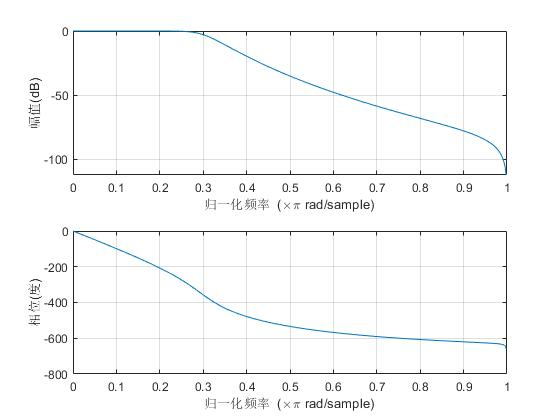
\includegraphics[width=1\textwidth]{"../DSPAssignment/冲激响应不变法.jpg"} %插入图片,[]中设置图片大小,{}中是图片文件名
	\caption{冲激响应不变法} %最终文档中希望显示的图片标题
	\label{Fig5} %用于文内引用的标签
\end{figure}
\begin{figure}[H] %H为当前位置,!htb为忽略美学标准,htbp为浮动图形
	\centering %图片居中
	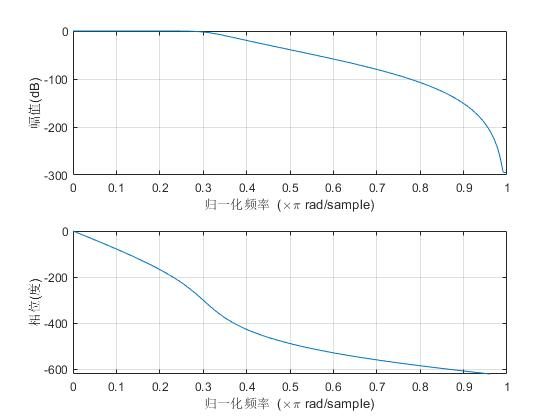
\includegraphics[width=1\textwidth]{"../DSPAssignment/双线性变换法.jpg"} %插入图片,[]中设置图片大小,{}中是图片文件名
	\caption{双线性变换法} %最终文档中希望显示的图片标题
	\label{Fig6} %用于文内引用的标签
\end{figure}
\subsection{结果分析}
\begin{enumerate}
	\item 冲激响应不变法- 优点:完全模仿模拟滤波器的单位冲激响应,即时域逼近良好;线性相位的模拟滤波器通过冲激响应不变法得到的仍为线性相位的数字滤波器。缺点:频率响应的混叠效应。
	\item 双线性变换法- 优点:避免了频率响应的混叠效应。	缺点:不再保持原有的线性相位,呈分段常数型;各个分段边缘的临界频率点产生了畸变。
\end{enumerate}
由 MATLAB 仿真结果可知,两种方法算出的模拟滤波器阶数以及截止频率均与理论计算结果相同,同时观察两者的频率特性响应图像也可以看出,数字滤波器的通带与阻带的衰减范围都符合一开始设定的数字指标要求,因此设计的 IIR 数字滤波器可以满足要求。 而两种方法也有
不同之处,如本实验中对于相同的数字指标,脉冲响应不变法比双线性变换法所得到的滤波器阶数更高,同时由于脉冲响应法的混叠影响,根据图像可以看出,脉冲响应不变法设计的低通滤波器相比于双线性变换法在过渡带下降比较平缓、特性较差。
\subsection{滤波器设计方法改进}
冲激响应不变法是从滤波器的单位抽样响应出发,使数字滤波器的单位抽样响应h(n)逼近模拟滤波器的单位抽样响应h(t),频率间的变化是线性变换关系,克服了双线性变换法中非线性频率变换带来的临界频率点的频率畸变,所以是最简单、最直接的把s平面映射到z平面的映射方法。但是该方法要求模拟滤波器是严格带限于抽样频率的1/2,如果不满足该要求,数字滤波器的频率响应将产生混叠失真。如果通过“模拟—模拟频带变换”方法设计IIR数字高通或者带阻滤波器,冲激响应法确实会产生混叠失真现象,但如果通过“数字—数字频带变换”方法则不存在该问题。因为该方法的数字化过程是将模拟低通滤波器的系统函数映射为数字低通滤波器的系统函数,而模拟低通滤波器是严格带限于抽样频率的1/2、是抗混叠的,所以不会出现频率混叠失真现象。
\\“数字—数字频带变换”的实质就是从数字低通滤波器的Z平面映射到另一个待求所需类型数字滤波器的z平面的变化关系,关键点是找到Z到z的映射函数$Z^{-1}=G(z^{-1})$。查阅资料可知,$
Z^{-1}=G\left(z^{-1}\right)=\frac{z^{-1}-\alpha}{1-\alpha^* z^{-1}} \cdot \frac{z^{-1}-\alpha^*}{1-\alpha z^{-1}}=\frac{z^{-2}+d_1 z^{-1}+d_2}{d_2 z^{-2}+d_1 z^{-1}+1}$,其中:$d_1=\frac{-2 \alpha}{1+k},d_2=\frac{1-k}{1+k},
k=\tan \left(\frac{\theta_p}{2}\right) \tan \left(\frac{\omega_{p_2}-\omega_{p_1}}{2}\right),
\alpha=\cos \left(\frac{\omega_{p_2}+\omega_{p_1}}{2}\right) / \cos \left(\frac{\omega_{p_2}-\omega_{p_1}}{2}\right)
$由Matlab仿真,使用由冲激响应不变法设计的带阻滤波器与用数字-数字频带变换设计的带阻滤波器比较,代码如下,仿真结果如图\ref{Fig7}、\ref{Fig8}所示。由结果对比图可以看出,通过冲激响应不变法完成模拟滤波器的数字化过程设计的带阻滤波器,确实存在频谱混叠失真,不符合设计参数,达不到设计要求。而采用数字-数字频带变换方法得到的带阻滤波器则不存在混叠现象,实现了对冲激响应法设计滤波器的改进。
\lstset{language=Matlab}
\begin{lstlisting}
	fp=0.2613*pi;fs=0.4018*pi;rp=0.75;rs=20;f=1; %设计指标
	wp1=fp*f;
	ws1=fs*f; %根据脉冲响应不变法变换数字滤波器到模拟滤波器指标
	[N1,wc1]=buttord(wp1,ws1,rp,rs,'s');%根据模拟指标设计巴特沃斯滤波器
	[B1,A1]=butter(N1,wc1,'s'); %得到传递函数
	[B3,A3]=lp2bs(B1,A1,wc1,0.2*pi);%由模拟低通转化为模拟带阻
	[num3,den3]=impinvar(B3,A3,f);%由模拟带阻转化为数字带阻
	freqz(num3,den3);%画出数字带阻滤波器频率响应
	bsp1=wc1-0.1*pi;bsp2=wc1+0.1*pi;%设置带阻滤波器阻带频率
	alpha=cos((bsp1+bsp2)/2)/cos((bsp2-bsp1)/2);
	klpha=tan((bsp1+bsp2)/2)*tan(wc1/2);
	d1=-2*alpha/(1+klpha);
	d2=(1-klpha)/(1+klpha);
	Nz=[d2,d1,1];
	Dz=[1,d1,d2];
	[num4,den4]=mapping(num1,den1,Nz,Dz);%根据数字-数字频带变换方法由数字低通变换为数字带阻
	freqz(num4,den4);%画出由数字-数字频带方法得到的带阻滤波器的频率响应
\end{lstlisting}
\begin{figure}[H] %H为当前位置,!htb为忽略美学标准,htbp为浮动图形
	\centering %图片居中
	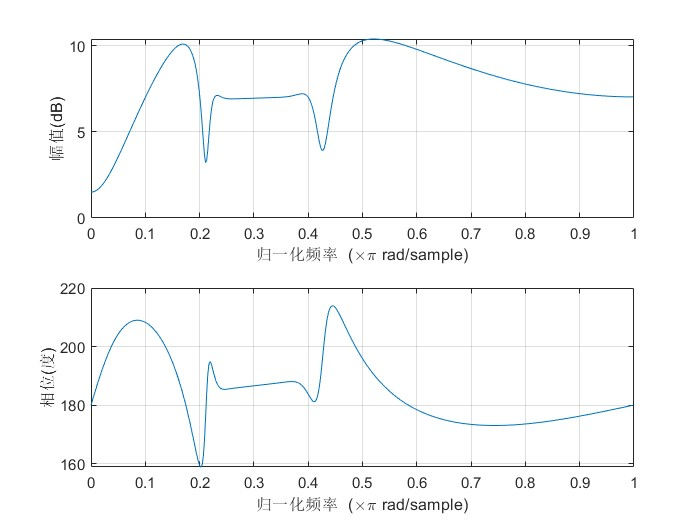
\includegraphics[width=1\textwidth]{"../DSPAssignment/带阻混叠.jpg"} %插入图片,[]中设置图片大小,{}中是图片文件名
	\caption{冲激响应不变法设计的带阻滤波器} %最终文档中希望显示的图片标题
	\label{Fig7} %用于文内引用的标签
\end{figure}
\begin{figure}[H] %H为当前位置,!htb为忽略美学标准,htbp为浮动图形
	\centering %图片居中
	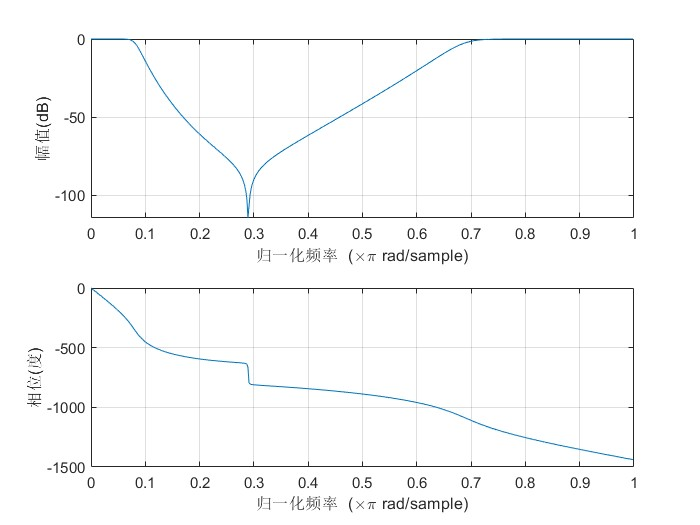
\includegraphics[width=1\textwidth]{"../DSPAssignment/带阻数字频带.jpg"} %插入图片,[]中设置图片大小,{}中是图片文件名
	\caption{数字-数字频带变换方法得到的带阻滤波器} %最终文档中希望显示的图片标题
	\label{Fig8} %用于文内引用的标签
\end{figure}
\end{document}
